\section{Recovering an Ellipsoid from Boundary Points}

For \(n=4\), write the symmetric matrix \(A\) as
\[
A=
\begin{bmatrix}
a_{11}&a_{12}&a_{13}&a_{14}\\
a_{12}&a_{22}&a_{23}&a_{24}\\
a_{13}&a_{23}&a_{33}&a_{34}\\
a_{14}&a_{24}&a_{34}&a_{44}
\end{bmatrix}
\]
For a sample \(x=(x_1,x_2,x_3,x_4)\), the equation \(x^TAx=1\) becomes
\[
a_{11}x_1^2
+2a_{12}x_1x_2
+2a_{13}x_1x_3
+2a_{14}x_1x_4
+a_{22}x_2^2
+2a_{23}x_2x_3
+2a_{24}x_2x_4
+a_{33}x_3^2
+2a_{34}x_3x_4
+a_{44}x_4^2
=1
\]
This is linear in the unknown entries of \(A\). Define
\[
\theta=
\begin{bmatrix}
a_{11}&a_{12}&a_{13}&a_{14}&a_{22}&a_{23}&a_{24}&a_{33}&a_{34}&a_{44}
\end{bmatrix}^T
\]
and form a row \(\phi(x)^T\) from the coefficients in the equation above. For all boundary samples,
\[
\Phi\theta\approx \mathbf{1}
\]
We can estimate \(\theta\) by least squares:
\[
\hat\theta=\arg\min_\theta \|\Phi\theta-\mathbf{1}\|_2^2
\]
Then we can reconstruct \(\hat A\) from the entries in \(\hat\theta\).

% For the data in \texttt{ellip\_bdry\_data.json}, \(n=4\) and \(N=100\). The recovered matrix is
% \[
% \hat A=
% \begin{bmatrix}
% 1.434950&0.050855&-2.870800&1.611960\\
% 0.050855&0.414349&-1.384180&0.898785\\
% -2.870800&-1.384180&16.136800&-11.844700\\
% 1.611960&0.898785&-11.844700&9.317230
% \end{bmatrix}
% \]
% Its eigenvalues are
% \[
% 0.046747,\qquad
% 0.421146,\qquad
% 1.233411,\qquad
% 25.602027
% \]

\begin{figure}[H]
    \centering
    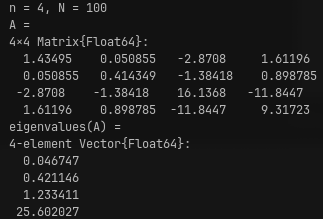
\includegraphics[width=0.4\textwidth]{img/p5a.png}
\end{figure}

All eigenvalues are positive, so \(\hat A>0\). Therefore
\[
\{x\in\mathbb{R}^4\mid x^T\hat A x=1\}
\]
is a genuine bounded ellipsoid.

To check consistency with the data, I computed
\[
r_k=(x^{(k)})^T\hat A x^{(k)}
\]
For exact boundary points, all \(r_k\) would equal one. In the data,
% \[
% \min_k r_k=0.697006,\qquad
% \max_k r_k=1.177020
% \]
% \[
% \frac{\|r-\mathbf{1}\|_2}{\sqrt{N}}=0.083636,
% \qquad
% \max_k |r_k-1|=0.302994
% \]

\begin{figure}[H]
    \centering
    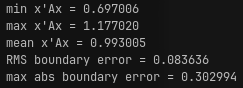
\includegraphics[width=0.4\textwidth]{img/p5b.png}
\end{figure}

The RMS boundary error and maximum absolute deviation are
\[
\frac{\|r-\mathbf{1}\|_2}{\sqrt{N}}=0.083636,
\qquad
\max_k|r_k-1|=0.302994
\]
Thus, a typical boundary value differs from \(1\) by about \(8.4\%\), and the largest deviation is approximately \(0.303\). These measures are more informative than the mean because positive and negative errors cannot cancel.

The mean value is
\[
\frac{1}{N}\sum_{k=1}^N r_k=0.993005
\]
The mean is close to \(1\), so the fit has little overall bias. Together with the positive eigenvalues of \(\hat A\), these errors indicate a reasonable fit to the noisy boundary data.

\subsection{Code}
\begin{lstlisting}[language={}]
using LinearAlgebra
using Statistics

include(joinpath(@__DIR__, "readclassjson.jl"))

function symmetric_design(X)
    n, N = size(X)
    pairs = Tuple{Int, Int}[]
    Phi = zeros(N, div(n * (n + 1), 2))

    col = 1
    for i in 1:n, j in i:n
        push!(pairs, (i, j))
        Phi[:, col] = i == j ? X[i, :] .^ 2 :
                               2 .* X[i, :] .* X[j, :]
        col += 1
    end

    return Phi, pairs
end

function symmetric_matrix(theta, pairs, n)
    A = zeros(n, n)
    for (col, (i, j)) in enumerate(pairs)
        A[i, j] = theta[col]
        A[j, i] = theta[col]
    end
    return Symmetric(A)
end

data = readclassjson(joinpath(@__DIR__, "ellip_bdry_data.json"))
X = data["X"]
n, N = size(X)

Phi, pairs = symmetric_design(X)
theta = Phi \ ones(N)
A = symmetric_matrix(theta, pairs, n)

values = [dot(X[:, k], A * X[:, k]) for k in 1:N]
errors = values .- 1
evals = eigvals(A)
\end{lstlisting}
